% !TeX program = lualatex
% ================================================================
% Polish Tier 3 Vocabulary Version of AlgebraStarters
%
% Generated by the server using the following settings:
%
%   language            Polish (pol)
%   text direction      left to right
%   font                Noto Serif
%   fallback font       Noto Serif
%   built from          latex/starters/retrieval/lessPriorKnowledge/algebraStarters.tex
%   vocabulary key      latex/starters/retrieval/lessPriorKnowledge/algebraStarters/L2/pol/algebraStarters_polishKey.tex
%   tier 3 vocabulary   green   RGB 0 128 0
%   English text        black   RGB 0 0 0
%   Polish text         purple  RGB 112 48 160
%   layout macros       version 3
%
% Please don't edit any information in this comment block - the server
% compares it against the current settings and rebuilds this file when
% they differ, so changes here would be overwritten. However, feel free
% to make updates to the LaTeX below if you want to edit it.
% ================================================================

\documentclass{beamer}
% ================================================================
% Copied from the English sheet this was translated from, so that
% anything it sets up for itself still works here
% ================================================================
\usepackage{tikz}
\usetikzlibrary{arrows.meta}
% ================================================================
% Answer-overlay helpers
% ================================================================
\newcommand{\ablank}[1]{%
  \alt<2>{\textcolor{red}{#1}}{\underline{\phantom{#1}}}%
}
\newcommand{\ashow}[1]{\uncover<2->{\textcolor{red}{\small #1}}}
\newcommand{\ashowq}[1]{\alt<2->{\textcolor{red}{\small #1}}{?}}

% Answers drawn straight on to a TikZ diagram, revealed on overlay 2 like \ashow.
% Space is reserved on overlay 1, so the diagram does not move between slides.
\usetikzlibrary{overlay-beamer-styles}
\tikzset{
  ans/.style     = {red, thick, visible on=<2->},
  ansfill/.style = {red!15, visible on=<2->},
  anslab/.style  = {red, font=\tiny, visible on=<2->},
}
\title{Year 8 Algebra Starters}
\date{}

% Characters this language's font has not got are borrowed from another,
% rather than being silently dropped - see docs/translated-sheet-latex.md
\directlua{%
  if luaotfload and luaotfload.add_fallback then
    luaotfload.add_fallback("eallatinfallback",
      { "Noto Serif:mode=harf;" })
  else
    tex.error("this luaotfload is too old to register a fallback font")
  end
}
\usepackage[english]{babel}
\babelprovide[import]{polish}
\babelfont[polish]{rm}[Renderer=Harfbuzz, BoldFont={Noto Serif}, ItalicFont={Noto Serif}, BoldItalicFont={Noto Serif}, RawFeature={fallback=eallatinfallback}]{Noto Serif}
\babelfont[polish]{sf}[Renderer=Harfbuzz, BoldFont={Noto Serif}, ItalicFont={Noto Serif}, BoldItalicFont={Noto Serif}, RawFeature={fallback=eallatinfallback}]{Noto Serif}
\newcommand{\ealtext}[1]{\foreignlanguage{polish}{#1}}
\newcommand{\ealtextblock}[1]{{\raggedright\foreignlanguage{polish}{#1}\par}}
% ================================================================
% EAL layout helpers
% ================================================================
\usepackage{xcolor}

\definecolor{ealkeycolour}{RGB}{0,128,0}
\definecolor{ealenglish}{RGB}{0,0,0}
\definecolor{ealtwocolour}{RGB}{112,48,160}

\newsavebox{\ealboxen}
\newsavebox{\ealboxtr}
\newlength{\ealglosswd}
\newlength{\ealglossraise}
\setlength{\ealglossraise}{1.15em}

% a tier 3 word, in English and in translation alike
\newcommand{\ealkey}[1]{\textcolor{ealkeycolour}{#1}}
\newcommand{\ealkeytr}[1]{\textcolor{ealkeycolour}{\ealtext{#1}}}

% One translated word above one English word. Built from kernel
% primitives, never a tabular, which would break wherever the sheet
% loads array, booktabs or tabularx. The box is as wide as the wider of
% the two, so a long translation pushes its neighbours aside instead of
% overlapping them, and it claims its full height so a table row or a
% TikZ node makes room for it.
\newcommand{\ealgloss}[2]{%
  \sbox{\ealboxen}{\ealkey{#1}}%
  \sbox{\ealboxtr}{\small\textcolor{ealtwocolour}{\ealtext{#2}}}%
  \setlength{\ealglosswd}{\wd\ealboxen}%
  \ifdim\wd\ealboxtr>\ealglosswd\setlength{\ealglosswd}{\wd\ealboxtr}\fi
  \leavevmode
  \makebox[\ealglosswd][c]{%
    \makebox[0pt][c]{\usebox{\ealboxen}}%
    \makebox[0pt][c]{\raisebox{\ealglossraise}{\usebox{\ealboxtr}}}%
  }%
}

% opens up line spacing around a block of glosses, so the raised
% translations sit clear of the line above
\newenvironment{ealglossed}{\par\linespread{2.1}\selectfont\ignorespaces}{\par}

% a whole translated sentence above its English counterpart. block level,
% so it does not belong inside a tabular cell
\newcommand{\ealpara}[2]{%
  \par\addvspace{0.5\baselineskip}%
  {\color{ealtwocolour}\ealtextblock{#1}}%
  \penalty200
  {\color{ealenglish}#2\par}%
  \addvspace{0.5\baselineskip}%
}

\begin{document}

\frame{\titlepage}

%------------------------------------------------
\begin{frame}{Starter 1}

\begin{ealglossed}
\begin{itemize}
  \item Calculate: $-5 + 12 =$ \ablank{$7$}
  \item Collect \ealgloss{like terms}{wyrazy podobne}: $3x + 4x =$ \ablank{$7x$}
  \item \ealgloss{Expand}{wymnażać nawiasy}: $3(x + 4) =$ \ablank{$3x+12$}
  \item Solve: $x + 6 = 14 \Rightarrow$ \ablank{$x=8$}
\end{itemize}

\vspace{0.3cm}

\begin{center}
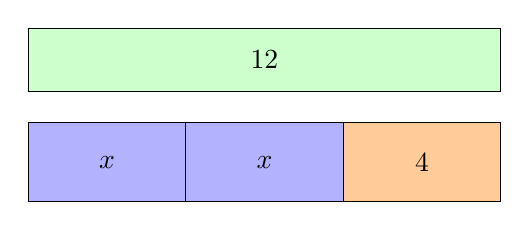
\begin{tikzpicture}
  \draw[fill=blue!30] (0,0) rectangle (2,1) node[midway] {$x$};
  \draw[fill=blue!30] (2,0) rectangle (4,1) node[midway] {$x$};
  \draw[fill=orange!40] (4,0) rectangle (6,1) node[midway] {$4$};
  \draw[fill=green!20] (0,1.4) rectangle (6,2.2) node[midway] {$12$};
\end{tikzpicture}
\end{center}

\begin{itemize}
  \item Write an \ealgloss{equation}{równanie} represented by the \ealgloss{bar model}{model słupkowy} and solve it. \ashow{$2x+4=12$, so $x=4$.}
  \item If the total was 18 instead of 12, what would $x$ be\ashowq{~$x=7$.}
  \item Is $3(x+4)=3x+4$ true or false? Explain. \ashow{False, because $3(x+4)=3x+12$.}
\end{itemize}
\end{ealglossed}

\end{frame}

%------------------------------------------------
\begin{frame}{Starter 2}

\begin{ealglossed}
\begin{itemize}
  \item Calculate: $6-11 =$ \ablank{$-5$}
  \item Collect \ealgloss{like terms}{wyrazy podobne}: $5x + 2 + 3x =$ \ablank{$8x+2$}
  \item \ealgloss{Expand}{wymnażać nawiasy}: $4(a + 2) =$ \ablank{$4a+8$}
  \item Solve: $2x = 14 \Rightarrow$ \ablank{$x=7$}
\end{itemize}

\vspace{0.3cm}

\begin{center}
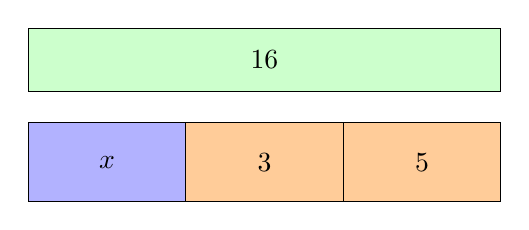
\begin{tikzpicture}
  \draw[fill=blue!30] (0,0) rectangle (2,1) node[midway] {$x$};
  \draw[fill=orange!40] (2,0) rectangle (4,1) node[midway] {$3$};
  \draw[fill=orange!40] (4,0) rectangle (6,1) node[midway] {$5$};
  \draw[fill=green!20] (0,1.4) rectangle (6,2.2) node[midway] {$16$};
\end{tikzpicture}
\end{center}

\begin{itemize}
  \item Write the \ealgloss{equation}{równanie} represented by the \ealgloss{bar model}{model słupkowy} and solve it. \ashow{$x+3+5=16$, so $x=8$.}
  \item Which part of the diagram represents the \ealgloss{constant}{stała}? \ashow{The $3$ and $5$ blocks (total $8$).}
  \item Create a \ealgloss{bar model}{model słupkowy} for $8x + 2 = 26$. \ashow{Eight $x$-blocks and a $2$-block, with total $26$.}
  \item Simplify: $ax + bx =$ \ablank{$(a+b)x$}
\end{itemize}
\end{ealglossed}

\end{frame}

%------------------------------------------------
\begin{frame}{Starter 3}

\begin{ealglossed}
\begin{itemize}
  \item Calculate: $-3 + 8 =$ \ablank{$5$}
  \item Collect \ealgloss{like terms}{wyrazy podobne}: $6a + 3 + 2a =$ \ablank{$8a+3$}
  \item \ealgloss{Expand}{wymnażać nawiasy}: $2(x + 7) =$ \ablank{$2x+14$}
  \item Solve: $x - 4 = 9 \Rightarrow$ \ablank{$x=13$}
\end{itemize}

\vspace{0.3cm}

\begin{center}
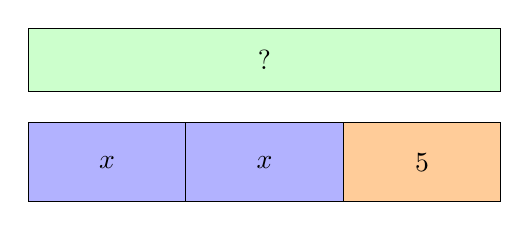
\begin{tikzpicture}
  \draw[fill=blue!30] (0,0) rectangle (2,1) node[midway] {$x$};
  \draw[fill=blue!30] (2,0) rectangle (4,1) node[midway] {$x$};
  \draw[fill=orange!40] (4,0) rectangle (6,1) node[midway] {$5$};
  \draw[fill=green!20] (0,1.4) rectangle (6,2.2) node[midway] {$?$};
\end{tikzpicture}
\end{center}

\begin{itemize}
  \item Suppose the total is 17. Write and solve the \ealgloss{equation}{równanie}. \ashow{$2x+5=17$, so $x=6$.}
  \item Suppose the total is 25. What is $x$ now\ashowq{~$x=10$.}
  \item \ealgloss{Expand}{wymnażać nawiasy}: $3(x+7) =$ \ablank{$3x+21$}
  \item \ealgloss{Expand}{wymnażać nawiasy}: $3(x-7) =$ \ablank{$3x-21$}
\end{itemize}
\end{ealglossed}

\end{frame}

%------------------------------------------------
\begin{frame}{Starter 4}

\begin{ealglossed}
\begin{itemize}
  \item Calculate: $-6 \div 3 =$ \ablank{$-2$}
  \item Collect \ealgloss{like terms}{wyrazy podobne}: $9a - 4a + 2 + 3b =$ \ablank{$5a+2+3b$}
  \item \ealgloss{Expand}{wymnażać nawiasy}: $5(y + 3) =$ \ablank{$5y+15$}
  \item Solve: $3d = 18 \Rightarrow$ \ablank{$d=6$}
\end{itemize}

\vspace{0.3cm}

\begin{center}
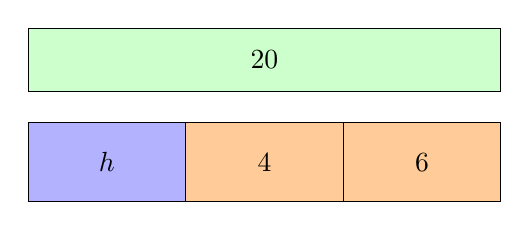
\begin{tikzpicture}
  \draw[fill=blue!30] (0,0) rectangle (2,1) node[midway] {$h$};
  \draw[fill=orange!40] (2,0) rectangle (4,1) node[midway] {$4$};
  \draw[fill=orange!40] (4,0) rectangle (6,1) node[midway] {$6$};
  \draw[fill=green!20] (0,1.4) rectangle (6,2.2) node[midway] {$20$};
\end{tikzpicture}
\end{center}

\begin{itemize}
  \item Write an \ealgloss{equation}{równanie} represented by the diagram and solve for $h$. \ashow{$h+4+6=20$, so $h=10$.}
  \item If the $4$ block was instead $h$ and the $h$ block was $4$, what \ealgloss{equation}{równanie} would we have\ashowq{~$4+h+6=20$.}
  \item \ealgloss{Expand}{wymnażać nawiasy}: $(x-3)(x-2) =$ \ablank{$x^2-5x+6$}
  \item Simplify: $a^2 \times a \times b =$ \ablank{$a^3b$}
\end{itemize}
\end{ealglossed}

\end{frame}

%------------------------------------------------
\begin{frame}{Starter 5}

\begin{ealglossed}
\begin{itemize}
  \item Calculate: $7 - 12 =$ \ablank{$-5$}
  \item Collect \ealgloss{like terms}{wyrazy podobne}: $2x + 7 + 3x =$ \ablank{$5x+7$}
  \item \ealgloss{Expand}{wymnażać nawiasy}: $3(a + 5) =$ \ablank{$3a+15$}
  \item Solve: $2x + 3 = 11 \Rightarrow$ \ablank{$x=4$}
\end{itemize}

\vspace{0.3cm}

\begin{center}
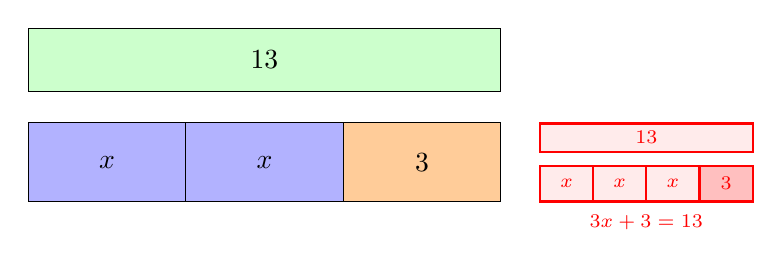
\begin{tikzpicture}
  \draw[fill=blue!30] (0,0) rectangle (2,1) node[midway] {$x$};
  \draw[fill=blue!30] (2,0) rectangle (4,1) node[midway] {$x$};
  \draw[fill=orange!40] (4,0) rectangle (6,1) node[midway] {$3$};
  \draw[fill=green!20] (0,1.4) rectangle (6,2.2) node[midway] {$13$};

% --- Q3 answer: a bar model for 3x + 3 = 13, drawn beside the given model ---
\begin{scope}[shift={(6.5,0)}, scale=0.45]
  \draw[ans, fill=red!8]  (0,1.4) rectangle (6,2.2)  node[midway, anslab, font=\scriptsize] {$13$};
  \draw[ans, fill=red!8]  (0,0) rectangle (1.5,1)    node[midway, anslab, font=\scriptsize] {$x$};
  \draw[ans, fill=red!8]  (1.5,0) rectangle (3,1)    node[midway, anslab, font=\scriptsize] {$x$};
  \draw[ans, fill=red!8]  (3,0) rectangle (4.5,1)    node[midway, anslab, font=\scriptsize] {$x$};
  \draw[ans, fill=red!25] (4.5,0) rectangle (6,1)    node[midway, anslab, font=\scriptsize] {$3$};
  \node[anslab, below, font=\scriptsize] at (3,-0.1) {$3x+3=13$};
\end{scope}
\end{tikzpicture}
\end{center}

\begin{itemize}
  \item Write and solve the \ealgloss{equation}{równanie} represented by the model. \ashow{$2x+3=13$, so $x=5$.}
  \item Explain how each part of the diagram matches the \ealgloss{equation}{równanie}. \ashow{Two $x$-blocks and a $3$-block make the total $13$.}
  \item Draw a \ealgloss{bar model}{model słupkowy} to represent $3x + 3 = 13$.
  \item Write an \ealgloss{equation}{równanie} with \ealgloss{solution}{rozwiązanie} $x=5$. \ashow{e.g.\ $x+2=7$.}
\end{itemize}
\end{ealglossed}

\end{frame}

%------------------------------------------------
\begin{frame}{Starter 6}

\begin{ealglossed}
\begin{itemize}
  \item Calculate: $-4 \times 6 =$ \ablank{$-24$}
  \item Collect \ealgloss{like terms}{wyrazy podobne}: $7x + 3x - 5 =$ \ablank{$10x-5$}
  \item \ealgloss{Expand}{wymnażać nawiasy}: $2(3x + 4) =$ \ablank{$6x+8$}
  \item Solve: $3x + 5 = 17 \Rightarrow$ \ablank{$x=4$}
\end{itemize}

\vspace{0.2cm}

\begin{itemize}
  \item Solve: $4x + 3 = 2x + 15 \Rightarrow$ \ablank{$x=6$}
  \item Solve: $\frac{x}{3} + 4 = 9 \Rightarrow$ \ablank{$x=15$}
\end{itemize}

\vspace{0.3cm}

\begin{center}
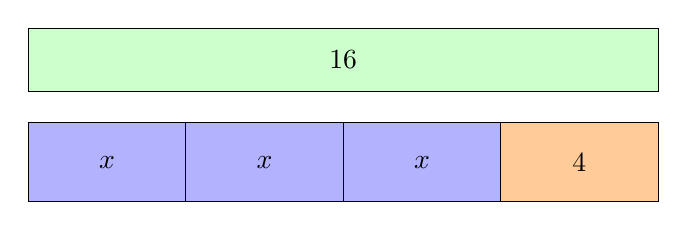
\begin{tikzpicture}

  \draw[fill=blue!30] (0,0) rectangle (2,1) node[midway] {$x$};
  \draw[fill=blue!30] (2,0) rectangle (4,1) node[midway] {$x$};
  \draw[fill=blue!30] (4,0) rectangle (6,1) node[midway] {$x$};
  \draw[fill=orange!40] (6,0) rectangle (8,1) node[midway] {$4$};
  \draw[fill=green!20] (0,1.4) rectangle (8,2.2) node[midway] {$16$};

\end{tikzpicture}
\end{center}

\begin{itemize}
  \item Write one \ealgloss{equation}{równanie} that could be represented by this \ealgloss{bar model}{model słupkowy}. \ashow{$3x+4=16$.}
  \item Write a different \ealgloss{equation}{równanie} with the same \ealgloss{solution}{rozwiązanie}. \ashow{e.g.\ $2x+3=11$.}
  \item Create an \ealgloss{equation}{równanie} with \ealgloss{solution}{rozwiązanie} $x=4$ that includes a \ealgloss{negative}{ujemny} \ealgloss{term}{wyraz}. \ashow{e.g.\ $2x-3=5$.}
\end{itemize}
\end{ealglossed}

\end{frame}

%------------------------------------------------

\end{document}